\subsection{Current and Previous Solutions}
\label{description:solution}
Currently Tomboy has the functionality to create bullet lists in Notes and with help of the Backlink Addin (which is shipped with the default Tomboy installation) to add Hyperlinks between different Notes. This allows the user to create simple task lists through Bulletlist and through linking a single task to another Note to create subtasks. This functionality is also shown in the GUI Mockup in Figure \ref{gui}.

% I commented this, so the information does not get lost to revisit this section.
% \subsubsection{Tasks} The idea of adding extended task management capability to Tomboy is not new and has been done before already:

% There is a project (realized as an Addin) for task management, called \textit{Tasks}, created by Boyd Timothy for quite some time. However, this was removed in Version 0.9.3 of Tomboy, because there were too many problems with the existing implementation\footnote{\url{http://lists.beatniksoftware.com/pipermail/tomboy-list-beatniksoftware.com/2008-January/000540.html}}, i.e. bugs and missing integration into Tomboy.
% %TODO: is this really that important? Yes, I think it shows how it was really too much a new application and not an Addin. Please remove this todo if you agree...
% Timothy abandoned the code and created a new program called \textit{Tasque}\footnote{\url{http://live.gnome.org/Tasque}} with its main focus just on task management.

% \subsubsection{TaskLists}
% In 2009 a new Addin was initiated by Sandy Armstrong. This unfinished project, called \textit{TaskLists}\footnote{\url{http://gitorious.org/~sandy/tomboy/sandys-tomboy/commits/task-lists2}} is still in a very early phase and has not much functionality yet. At the moment nobody is regularly working on it.

% \subsubsection{Others}
% Also, there are various inofficial Addins that all have only a very small part of the functionality that we would like to implement. Examples are the \textit{Tomboy-Todo}
% Addin \footnote{\url{http://romain.blogreen.org/Projects/Tomboy-Todo}} and the \textit{tasklist} Addin\footnote{\url{http://www.ediweissmann.com/taskslist/}}.

% \subsubsection{Conclusion}

\label{integration}
In the past, there have been several official\footnote{\url{http://lists.beatniksoftware.com/pipermail/tomboy-list-beatniksoftware.com/2008-January/000540.html}}$^,$\footnote{\url{http://gitorious.org/~sandy/tomboy/sandys-tomboy/commits/task-lists2}} and inofficial (e.g.\footnote{\url{http://www.ediweissmann.com/taskslist/}}) attempts to come up with an Addin for handling tasks in Tomboy which however all did not result in a satisfactory end product due to missing functionality or integration.

Our goal is to finish such a project up to a stable and working solution (in terms of \textit{bug-freeness} and \textit{usability}) that is fully integrated into Tomboys existing concepts and easy and simple to use, such that it could hopefully accepted to be included in the Tomboy project and shipped with future Tomboy releases.

\subsection{Product Perspective}
\label{description:perspective}
  The project TaskManager for Tomboy will be part of the Tomboy project.\\
  Figure \ref{perspective} shows the Product perspective of the TaskManager Addin. Since it's really an extension for Tomboy it is placed in
  the Addins section of Tomboy itself where it will communicate with some of Tomboys internal elements (as shown by connecting lines).
  \begin{itemize}
    \item TaskManager will directly customize the Tomboy NoteWriter user interface in a way that the user can write task lists in notes 
	(this functionality can be seen in Figure \ref{gui}. To achieve this TaskManager will  directly rely on some of the 
	Widgets in the GTK\# library. The corresponding requirements for this are documented in section \ref{requirements:interfaces:user}.
    \item On the other hand notes have to be made persistent. Since we introduce an additional concept in notes (mainly
    the notion to write tasks in notes) we have to save the task information by using the storage facilities available by Tomboy and probably extend
    the currently available XML format to store notes. This functionality is covered in requirements \ref{??}%TODO.
    \item Last but not least TaskManager will give the user a way find notes with open tasks or tasks that are overdue. This means we have to modify
    the existing Note Browser user interface. This functionality is covered in requirements \ref{??}%TODO.
  \end{itemize}


  
 
  \begin{figure}[ht]
    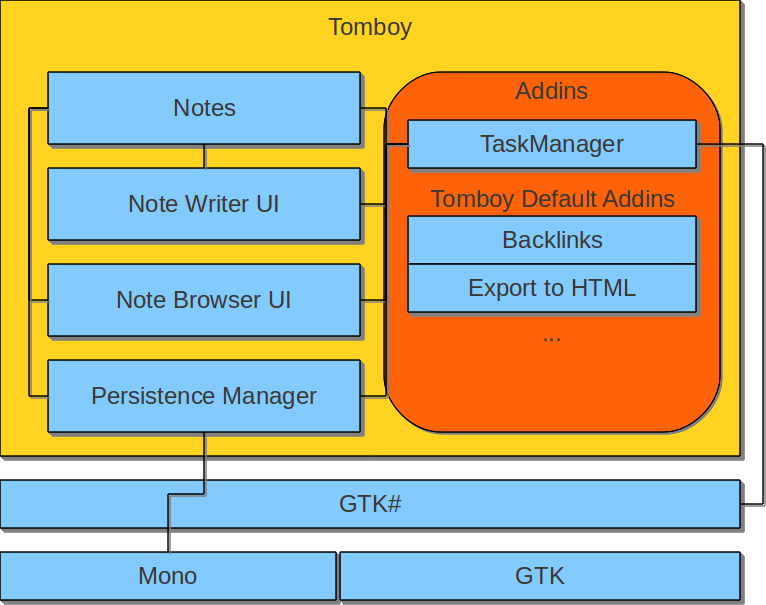
\includegraphics[width=\textwidth]{graphics/product_perspective_diagram.png}
    \caption{TaskManager Product Perspective}
    \label{perspective}
  \end{figure}


\subsection{Product Functions}
\label{description:functions}

  \subsubsection*{Supported Functions}
  \label{description:functions:supported}

    \begin{itemize}
      \item Provides advanced Task management capabilities for Tomboy
      \item Allows multiple tasks to be grouped together
      \item Supports priorities and due dates for tasks
      \item Allows to establish relationships/dependencies between tasks
      \item Allows the user to conveniently get to the tasks currently not finished/finished or overdue.
      \item Allows to export all defined tasks
    \end{itemize}

    \subsubsection*{Unsupported Functions}
      \label{description:functions:unsupported}
      \begin{itemize}
        \item Does not introduce additional GUI window elements or external tools within or outside of Tomboy (see \ref{integration} for the reason of that).
          %TODO: Is this really a 'function'(ality)? Yes, according to \ref{integration}. Please remove this todo if you agree...
        \item Does not support on-the-fly synchronization with external tools or clients except for manual export.
        \item Does not support importing tasks from other Task manager tools.
      \end{itemize}

\subsection{User Characteristics}
\label{description:usercharacteristics}
We look at two types of users:

  \begin{itemize}
    \item[\bf{Casual}] The casual user will create simple task lists. He may not know the various functions of Tomboy very well. Still, he should be able to create simple task lists where he can cross out individual elements easily.

    \item[\bf{Advanced}] The advanced user knows and uses Tomboy already quite well. He should be able to add arguments such as due dates and priorities to his task lists, create hierarchies of tasks and may export his lists to other tools such as \textit{Evolution} without much effort.
  \end{itemize}


\subsection{Constraints}
\label{description:constraints}
The Addin itself should obey all criterias (standards and guidelines) imposed by the GNOME and Tomboy projects (Tomboy Styleguide, \ref{styleguide}).

Besides the coding guidelines this includes mainly design aspects, such as simplicity and easyness of use, and full integration into Tomboy (see also \ref{integration}).


\subsection{Assumptions and Dependencies}
\label{description:assumptions}
